\documentclass[journal]{vgtc}                % final (journal style)
%\documentclass[review,journal]{vgtc}         % review (journal style)
%\documentclass[widereview]{vgtc}             % wide-spaced review
%\documentclass[preprint,journal]{vgtc}       % preprint (journal style)
%\documentclass[electronic,journal]{vgtc}     % electronic version, journal

%% Please note that the use of figures other than the optional teaser is not permitted on the first page
%% of the journal version.  Figures should begin on the second page and be
%% in CMYK or Grey scale format, otherwise, colour shifting may occur
%% during the printing process.  Papers submitted with figures other than the optional teaser on the
%% first page will be refused.

\usepackage{mathptmx}
\usepackage{graphicx}
\graphicspath{{./images/}}
\usepackage{times}
\usepackage{natbib}
\usepackage{booktabs}
\usepackage{amsmath}
\usepackage{mathtools}

%% This turns references into clickable hyperlinks.
\usepackage[bookmarks,backref=false,linkcolor=black]{hyperref} %,colorlinks
\hypersetup{
  pdfauthor = {},
  pdftitle = {},
  pdfsubject = {},
  pdfkeywords = {},
  colorlinks = true,
  linkcolor = black,
  citecolor = black,
  pageanchor = true,
  urlcolor = black,
  plainpages = false,
  linktocpage
}

%% If you are submitting a paper to a conference for review with a double
%% blind reviewing process, please replace the value ``0'' below with your
%% OnlineID. Otherwise, you may safely leave it at ``0''.
\onlineid{0}

%% declare the category of your paper, only shown in review mode
\vgtccategory{Research}

%% allow for this line if you want the electronic option to work properly
% \vgtcinsertpkg

%% In preprint mode you may define your own headline.
%\preprinttext{To appear in an IEEE VGTC sponsored conference.}

%% Paper title.

\title{Bin-summarise-smooth: A framework for visualising large data}

%% indicate IEEE Member or Student Member in form indicated below
\author{Hadley Wickham}
\authorfooter{
%% insert punctuation at end of each item
\item
 Hadley Wickham is Chief Scientist at RStudio. E-mail: h.wickham@gmail.com.
}

%other entries to be set up for journal
\shortauthortitle{Wickham: A visualisation framework for in-memory big data}

%% Abstract section.
\abstract{

Visualising large data is challenging both perceptually and computationally: it is hard to know what to display and hard to efficiently display it once you know what you want. This paper outlines a framework to tackle both problems, based around a four step process of bin, summarise, smooth, and visualise. Binning and summarising efficiently (O(n)) condense the large raw data into a form suitable for display (recognising that there are $\sim 3$ million pixels on a screen). Smoothing helps resolve problems from binning and summarising, and because it works on smaller, condensed datasets, it can make of use algorithms that are more statistical efficient even though they're more computationally expensive.

The paper is accompanied by single-core in-memory reference implementation that produces static graphics in R, the {\tt bigvis} package. The framework is readily extensible to parallel out-of-memory solutions, and to interactive and dynamic graphics.
} 

%% Keywords that describe your work. Will show as 'Index Terms' in journal
%% please capitalize first letter and insert punctuation after last keyword
\keywords{Big data, kernel smoothing.}

%% ACM Computing Classification System (CCS). 
%% See <http://www.acm.org/class/1998/> for details.
\CCScatlist{ % not used in journal version
  \CCScat{I.5.1}{Pattern recognition}{Models}{Statistical};
  \CCScat{G.3}{Probability and statistics}{Statistical computing};
}

\teaser{
  \centering
  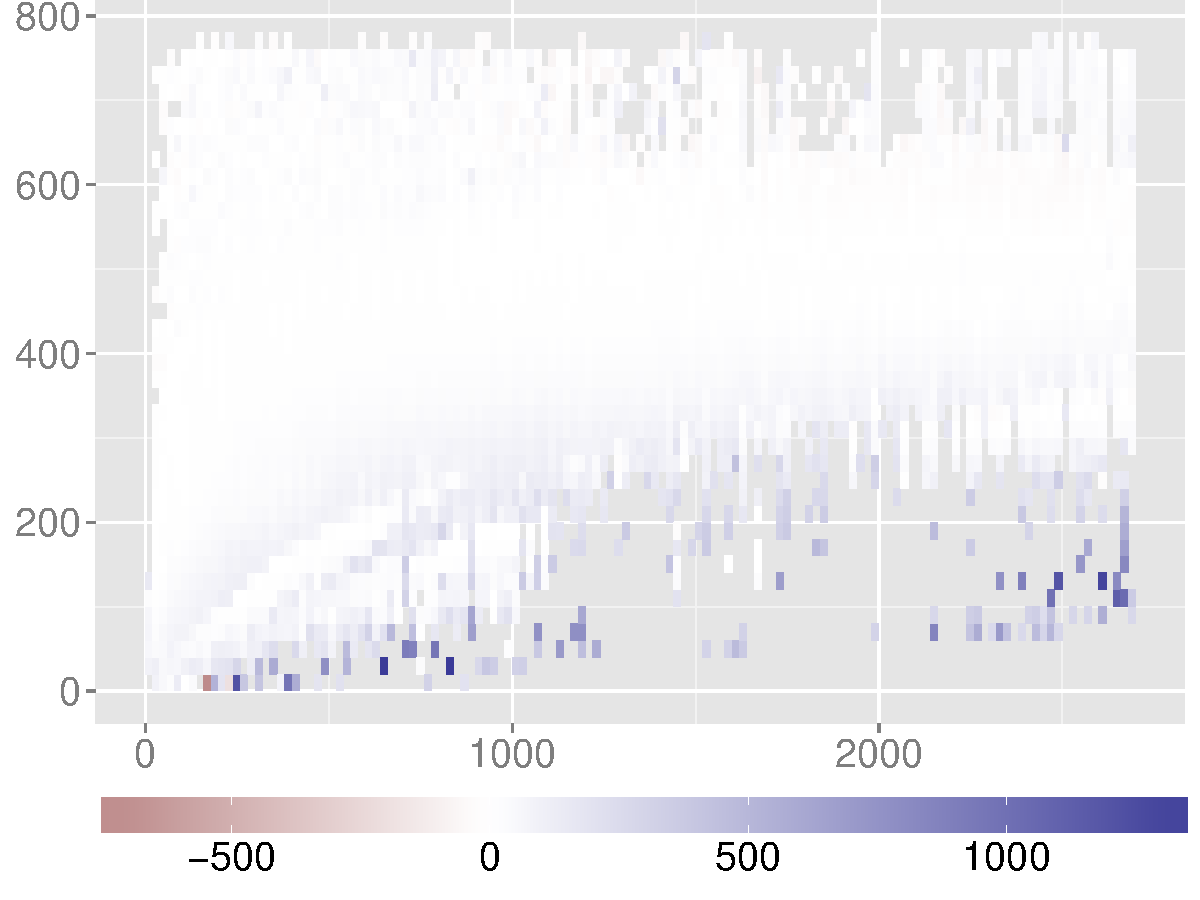
\includegraphics[width=5.33cm]{teaser-1}%
  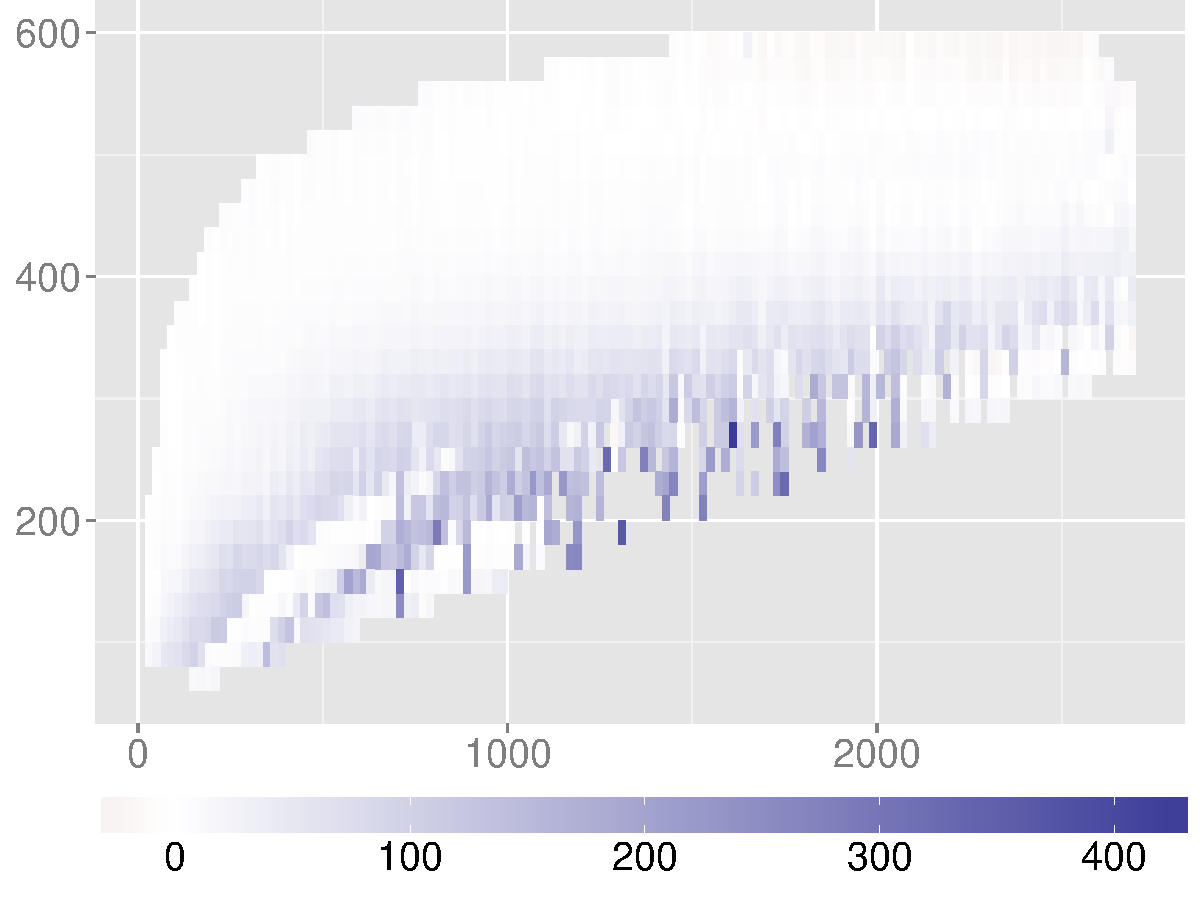
\includegraphics[width=5.33cm]{teaser-2}%
  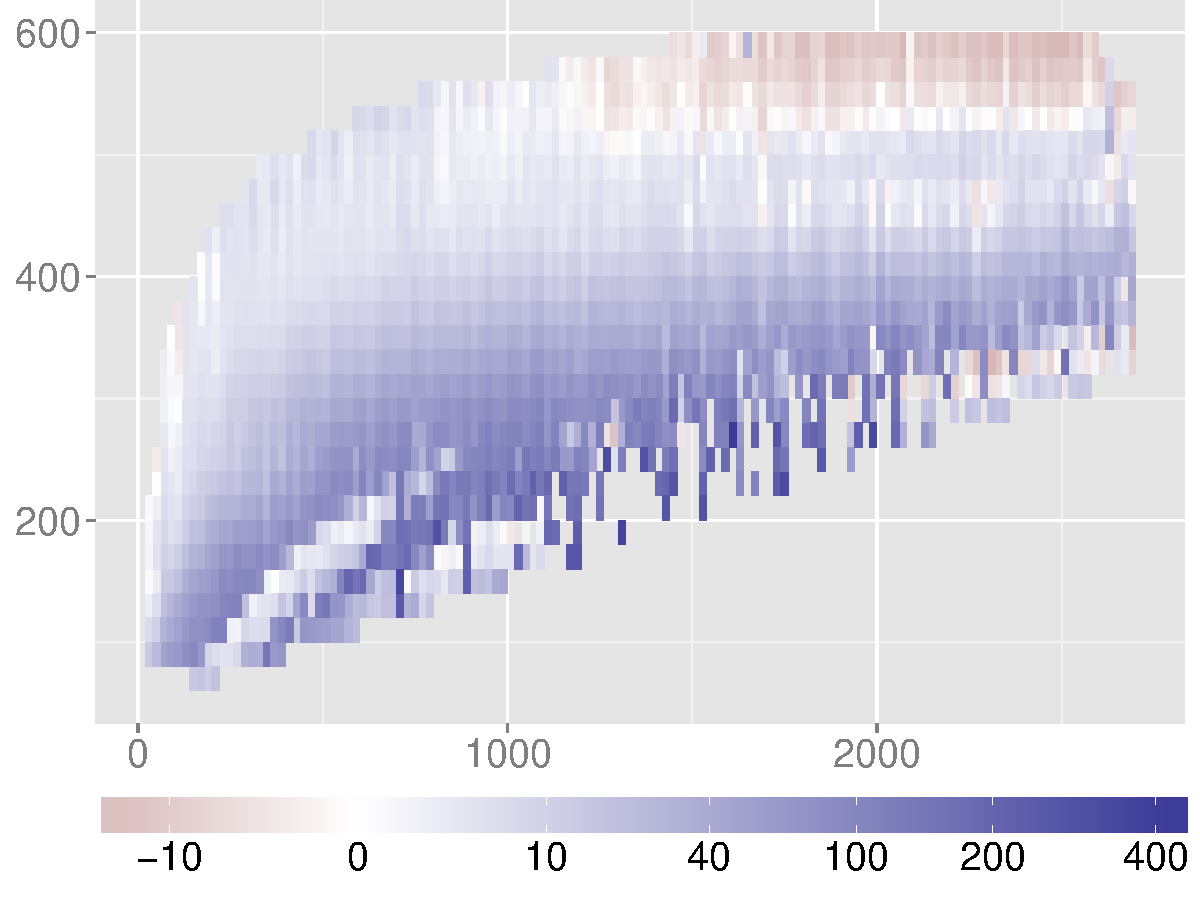
\includegraphics[width=5.33cm]{teaser-3}
  \caption{Average delay (colour, in minutes) as a funtion of distance (x axis, in miles) and speed (y axis, in mph) for 76 million flights. The visualisation needs refinement to be useful: (Left) all data, (center) focussing on the middle 99.5\% of the data, (right) transforming average delay to shrink the tails and focus on values near 0. Flights with higher than average speeds (top-right) have shorter delays (red); more interestingly, a subset of shorter, slower flights (bottom-left) have average delays close to 0 (white).}
  \label{fig:teaser}
}


%%%%%%%%%%%%%%%%%%%%%%%%%%%%%%%%%%%%%%%%%%%%%%%%%%%%%%%%%%%%%%%%
%%%%%%%%%%%%%%%%%%%%%% START OF THE PAPER %%%%%%%%%%%%%%%%%%%%%%
%%%%%%%%%%%%%%%%%%%%%%%%%%%%%%%%%%%%%%%%%%%%%%%%%%%%%%%%%%%%%%%%%

\begin{document}
\firstsection{Introduction}

\maketitle

As data grows ever larger, it is important that our ability to visualise it grows too. This paper presents a novel framework for visualising large data that is designed to be both computationally and statistically efficient, dealing with both the challenges of what to display for very large datasets and how to display it fast enough for interactive exploration. The insight that underlies this work is simple: the bottleneck when visualising large datasets is the number of pixels on a screen. At most we have around 3,000,000 pixels to use, and 1d summaries need only 3,000 pixels. There is no point displaying more data than pixels, and rathering than relying on the rendering engine to intelligently reduce the data, we develop summaries built on well-known statistical principles. 

The framework includes the most important 1d and 2d statistical graphics: histograms, frequency polygons and kernel density estimates for 1d data; scatterplots, scatterplot smoothers and boxplots. 

It is readily extensible to new visualisations that instead focus on higher moments (like standard deviation, skewness and kurtosis) instead of the mean or median.

The framework attempts to address the tension between a providing flexible system that can that doesn't restrict the analyst to preconcieved visualisations, but equally is constrained to a domain where computation can be performed efficiently. 

The framework involves four steps: binning, summarising, smoothing and visualising. Binning and summarising condenses the large raw data to a summary on the same order of size as pixels on the screen. To be computational efficient, binning and summarising make some statistical sacrifices, but but these can be compensated for with the smoothing step. Smoothing is computationally harder, but smoothing condensed data is fast and looses little statistical strength. 

Section \ref{sec:condense} discusses binning and summarising, focussing on the computational concerns. Computationally, we want linear behaviour and the ability to parallelise, but statistically, we want summaries that are resistant to unusual values. Section~\ref{sec:smooth} discusses smoothing, focussing more on the statistical side, and shows how we can remedy some of the statistical problems with the fast binning and summary steps. Even once we've reduced the data to manageable size, visualisation of large data presents some special challenges. In Section~\ref{sec:visualise}, we discuss generally how to visualise the condensed datasets, and some of the particular problems with very large data, notably problems caused ``unusual'' values.  

The paper is accompanied by an open-source reference implementation in the form of the bigvis R \citep{R} package. This is available from \url{http://github.com/hadley/bigvis} and is described in Section~\ref{sec:bigvis}. While the reference implementation focusses on in-memory, single-core summaries of continuous data with an eye to produce static graphics, these are not limitations of the framework, and while not the focus of the paper, I will also mention issues with out-of-memory data, parallel multi-core processing and interactive visualisations. 

To illustrate the framework I include figures generated from the flight on-time performance data made available by the Bureau of Transporation Statistics\footnote{\url{http://transtats.bts.gov/Fields.asp?Table_ID=236}}. I use flight performance data for all domestic US flights 2000--2011: $\sim$78,000,000 flights in total. The complete dataset has 111 variables, but here we'll explore just four: the flight distance (in miles), elapsed time (in minutes), average speed (in mph) and the arrival delay (in minutes). The data was mildly cleaned: negative times, speeds greater 761 mph (the speed of sound), and distances greater than 2724 miles (the longest flight in the continental US, {\sc sea}--{\sc mia}) were replaced with missing values. This affected $\sim$1.8 million (2.4\%) rows. The data, and code, needed to reproduce this paper and accompanying figures can be found at \url{http://github.com/hadley/bigvis}.

\section{Related work}
\label{sec:related-work}

% Related statistics work
There is an extensive body of statistical research on density estimation (smooth histograms) and smoothing, stretching back to the early 70s. Three good summaries of the work are \cite{scott:1992,bowman:1997,loader:1999a}.    \cite{hardle:1992,wand:1994,fan:1994} focus on the computational side of the smooth estimators, much of which occured in the early 90s as statisticians worked to transition their algorithms from mainframes to PCs.  Surprisingly none recognise that simple kernel smoothing is a convolution, and in high-dimensions rearranging the order of the convolution can change the problem from $O(n^d)$ to $O(nd)$. But these papers only treat special cases of this framework, fail to treat some of the problems associated with visualising large data and are not accompanied by code.

% Infovis and kde
\citep{lampe:2011} uses kernel density estimates in an infovis context, but fails to connect their work to existing statistical work. Provide a very fast implementation on the GPU, which presumably could be made even faster if they read previous work. Other techniques from infovis are related to kernel density estimation. Footprint splatting \citep{becker:1997,yang:2003} is exactly equivalent to kernel density estimation. Similarly, using transparency as a way of dealing with overplotting, as in ..., can be seen as a special type of kernel density estimate where the kernel is a uniform radial point.

% Other papers on large data
There are other techniques to deal scatterplots of large data. Hexbin plots \citep{carr:1987} bin 2d data using hexagons to avoid the perceptual issues related to gridding. Generalised scatterplots \citep{keim:2010} use distortion, but no discussion of computational performance. \citep{heer:2012} discusses the challenges of visualising large data, and proposes interaction as a solution. Emphasises the challenge of data cleaning and manipulation.

\citep{unwin:2006} aggregates much work from statistical graphics.


\section{Condense}
\label{sec:condense}

The first step in the framework is to condense the large original dataset to binned summaries which we will later visualise. Figure~\ref{fig:condense} illustrates the principle with the distance variable. Distance is binned in to 10-mile-wide bins, and each bin is summarised with three counts: the count, the average speed, and the standard deviation of the speed. To do this we first assign each observation to an integer bin, as described in Section~\ref{sub:bin}; and then reduce all observations in a bin to a handful of summary statistics, as described in Section~\ref{sub:summarise}.

\begin{figure}[htb]
 \centering
 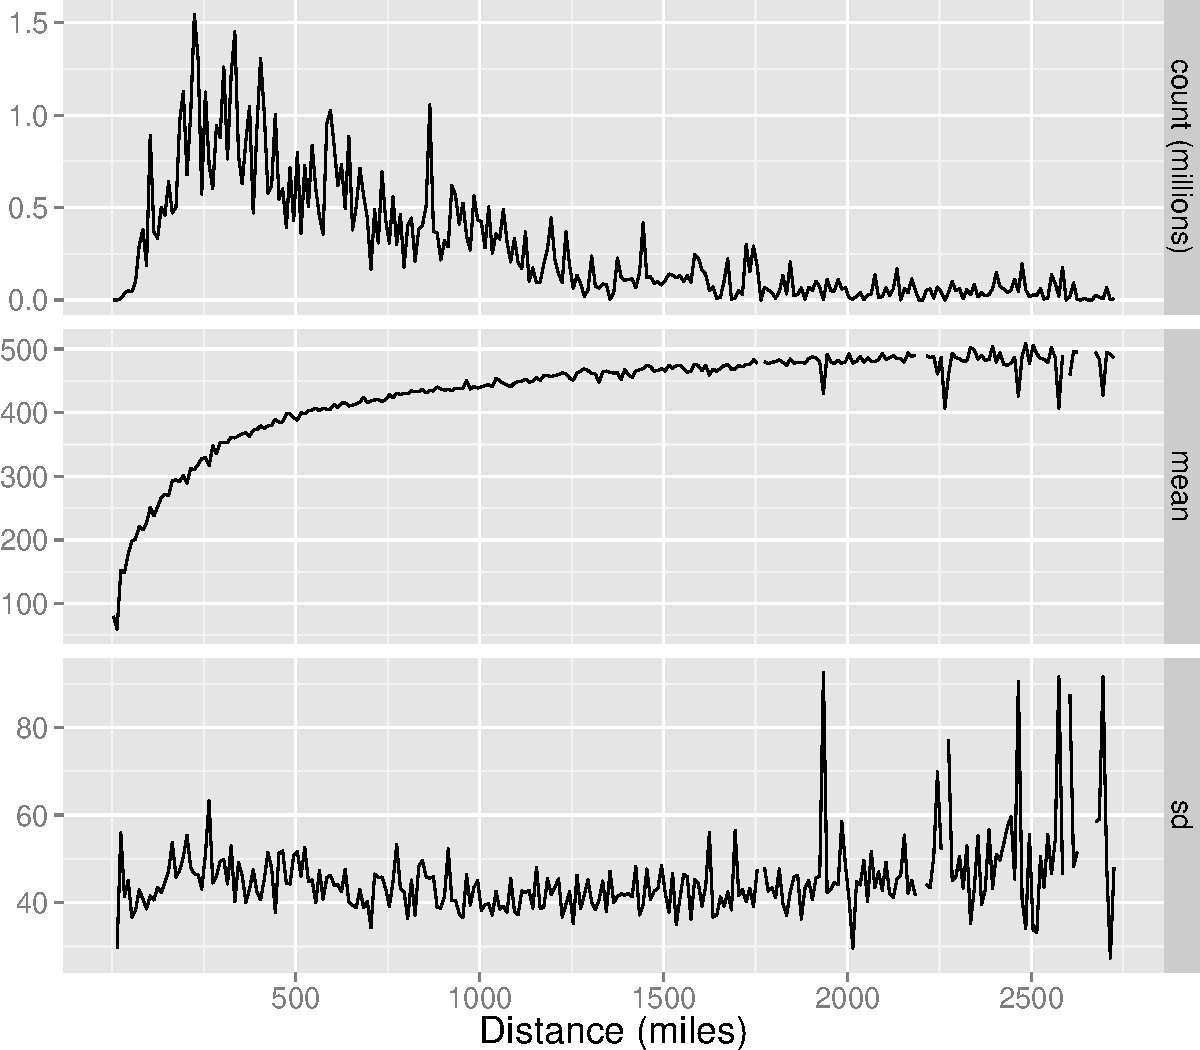
\includegraphics[width=\linewidth]{condense}
 \caption{Distance binned into 273 10-mile-wide bins, summarised with count, mean speed and standard deviation of speed. Note the varying scales on the y-axis.}
 \label{fig:condense}
\end{figure}

\subsection{Bin}
\label{sub:bin}

We first assign each observation to an integer representing a bin. We want an injective mapping, so that many data points will be mapped to a single integer.
We use {\bf fixed width binning}. Fixed width binning is extremely computationally efficient, easily extended from 1d to nd, and while statistically na\"ive, there is little evidence that variable binwidths do better. 

It is important to think of binning as a separate step, as it may be performed outside of the visualisation environment, for example in the database layer (integers require half as much space as doubles, so this could half data transmission costs). 

\subsubsection{Computation}

Fixed width binning is parameterised by two variables, the origin (the position of the first bin) and the width. The computation is shown in \eqref{eq:fixed-width}.

\begin{equation}
  \label{eq:fixed-width}
  \left \lfloor \frac{x - \text{origin}}{\text{width}} \right \rfloor + 1
\end{equation}

Bins are 1-indexed, reserving bin 0 for missing values and values smaller than the origin.

\subsubsection{Extension to nd}

Fixed width binning can be easily extended to multiple dimensions. You first bin each dimension, producing a vector of integers $(x_1, x_2, ..., x_m)$. It is then straightforward to devise a bijective map between this vector and a single integer, given that we know the largest bin in each dimension. If we have $m$ dimensions, each taking possible values $0, 1, \ldots, n_m$, then we can collapse the vector of integers into a single integer using this formula:

\begin{equation}
  \label{eq:nd-bins}
  \begin{matrix*}[l]
   = & x_1 + x_2 \cdot n_1 + x_3 \cdot n_1 \cdot n_2 + \cdots + x_m * \Pi^{n-1}_{i = 1} n_i \\
   = & x_1 + n_1 \cdot (x_2 + n_2 \cdot (x_3 + \cdots(x_m))
  \end{matrix*}
\end{equation}

It is easy to see how this works if each dimension has ten bins. For example, to project 3d bin $(5, 0, 4)$ into 1d, we compute $5 + 0 * 10 + 4 * 100 = 4 + 10 * (0 + 10 * 5) = 405$. Given a single integer, we can find the vector of $m$ original bins by reversing the transformation, peeling off the integer remainder after dividing by 10. For example, 1d bin $356$ corresponds to 3d bin $(6, 5, 3)$.

This function is a monotone minimal perfect hash, and highly efficient hashmap variants are available that make use of its special properties \citep{belazzougui:2009}. For example, because the hash is perfect, we can eliminate the equivality comparison that is usually needed after a candidate has been found with the hashed value. Even if this data structure is not used (as in the reference implementation), it easy to efficiently summarise bins in high-dimensions using standard data structures: either a vector if most bins have data in them, or a hashmap if not.

The challenges of working with nd summaries are typically perceptual, rather than computational. Figure~\ref{fig:condense-2d} shows a 2d summary of distance and speed: even moving from 1d to 2d makes it significantly harder to accurately percieve count \citep{cleveland:1984}.

\begin{figure}[htb]
 \centering
 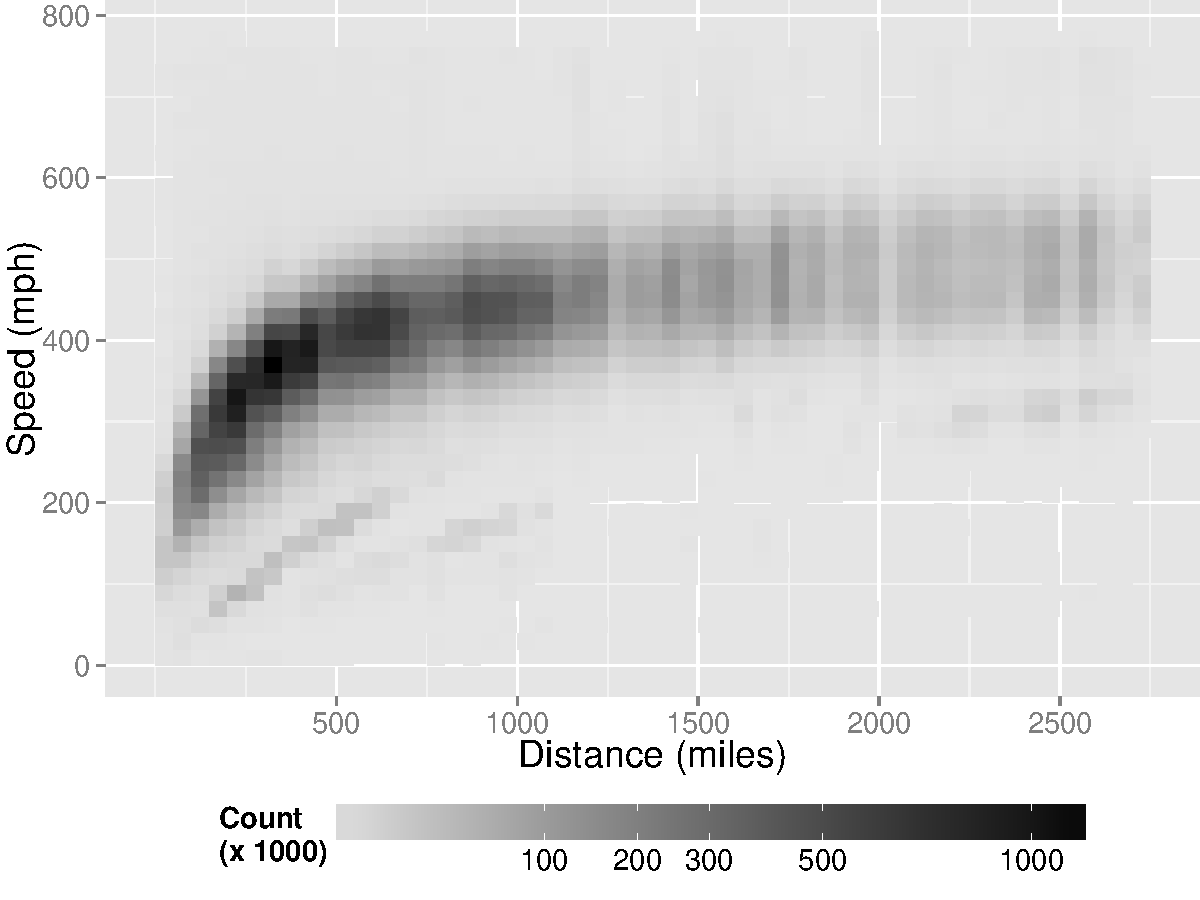
\includegraphics[width=\linewidth]{condense-2d}
 \caption{Distance and speed summarised with count. Note that count scale has been transformed slightly, as described in Section~\ref{sub:transform}, to draw attention to regions with fewer counts.}
 \label{fig:condense-2d}
\end{figure}

\subsubsection{Statistical limitations}

Ideally, we would like bigger bins in regions with few data points because the error of the summary is typically $\Theta(1 / \sqrt{n})$. For example, in Figure~\ref{fig:condense} we would like to have bigger bins for larger distances since the counts are small and the estimates of mean and standard deviation are more variable than we would like. However, there is little evidence that varying binwidths leads to asymptotically lower error \citep{terrell:1992}; while varying bin widths should provide a better approximation to the underlying data, the optimisation problem is so much more challenging that any potential improvements are lost. Instead of resolving these issues with a more sophisticated binning algorithm, we will fix them in the later smoothing step.  

% Linear binning vs. simple binning

% proviso that the bin is a integer, so can not store more than $2^32$ possible bins. (This seems like a lot but shrinks quickly as the number of dimensions grows: it's 85 bin in each direction in 5d and only 9 bins in each direction in 10d).  Outside that range can switch to standard hashing algorithms, albeit with a performance penalty because the algorithm will be more complex, and additional equality comparisons will be required. (Read citations on \url{http://en.wikipedia.org/wiki/Perfect_hash_function} and cite appropritately)

\subsection{Summarise}
\label{sub:summarise}

Once each of the $n$ original data points has been placed into one of $m$ integer bins ($m \ll n$), the next step is to collapse the points in each bin into a small number of summary statistics. Picking useful summary statistics requires balancing between computational efficiency and statistical robustness. 

\subsubsection{Computationl efficiency}

Gray et al. \citep{gray:1997} provide a useful classification for understanding the computational characteristics of a summary statistic. A summary is:

\begin{itemize}
  \item {\bf distributive} if it can be computed using a single element of interim storage and summaries from subgroups can be combined. This includes count, sum, min, and max.
  
  \item {\bf algebraic} if it is a combination of a fixed number of distributive statistics. This includes the mean (count + sum), standard deviation (count + sum + sum of squares) and higher moments like skewness and kurtosis.
  
  \item {\bf holistic} if it requires interim storage that grows with the input data. This includes quantiles (like the median), count of distinct elements or the most common value. 

\end{itemize}

Algebraic and distributive statistics are important because results from subgroups can easily be combined. This has two benefits: it makes parallelisation trivial, and it supports a tiered approach to exploration. For example, if you have 100 million observations, you might first finely bin into 100,000 bins. Then for any specific 1d plot, you rebin or subset the fine bins rather than the original data. This tiered approach is particularly useful for interactive visualisations; the fine binning can be done upfront when the visualisation is created, then modifying the binwidth or plot limits can be done interactively.

It is often possible to convert a summary from holistic to algebraic by taking an approximation. For example, the count of distinct values can be approximated with the hyperloglog algorithm \citep{flajolet:2007}, the median with the remedian \citep{rousseeuw:1990}, and other quantiles with other methods \citep{finkelstein:1994,hurley:1995,liechty:2003}. Others have proposed general methods for approximating any holistic summary \citep{christmann:2007}.

The mean, standard deviation and higher moments can all be computed in a single pass, taking $O(n)$ time and $O(1)$ memory. Some care is needed as naive implementations (e.g.\ computing the variance as $\sum_i^n x_i^2 / n - \left( \sum_i^n x_i / n \right)^2$) can suffer from severe numerical problems, but better algorithms are well known \citep{welford:1962}. The median also takes $O(n)$ time (using the quick-select algorithm), but needs $O(n)$ memory: there is no way to compute the median without storing at least half of the data, and given the median of two subgroups, no way to compute the median of the full dataset.

\subsubsection{Statistical robustness}

There is an interesting tension between the mean and the median: the median is much more robust to unusual values than the mean, but requires unbounded memory. A useful way to look at the robustness of a statistic is the {\bf breakdown point}. The breakdown point of a summary is the proportion of observations an attacker needs to control before they can arbitrarily influence the resulting summary. It is 0 for the mean: if you can influence one value, you can force the mean to be any value you like. The breakdown point for the median is 0.5: you have to taint 50\% of the observations before you can arbitrarily change the median. The mean is computationally desirable, but is less statistically desirable since just one flawed value can arbitrarily taint the summary. This is a general problem: the easiest summary statistics to compute are also the least robust, while robust statistics are usually holistic.

Even if you do use robust statistics, you are only protected from scattered outliers, not a radical mismatch between the data and the summary. For example, a single measure of central tendency (mean or median) will never be a good summary if the data has multiple modes. Compare Figures~\ref{fig:condense} and \ref{fig:condense-2d}: for shorter flights, there appears to be multiple modes of speed for a given distance and so the mean is not a good summary. Visualisation must be iterative: you can not collapse a variable to a single number until you have some confidence that the summary isn't throwing away important information. In practice, users may need to develop their own summary statistics for the pecularities of their data; the ones discussed here should provide a good start for general use.

\subsubsection{Higher dimensions}

There is no reason to limit ourselves to only 1d summary functions. 2d summaries like the correlation may also be interesting. All statistics from a linear model can be computed in $O(n)$ in time and $O(1)$ in space \citep{miller:1992}, and are and thus suggest a fruitful ground for generalisations to higher dimensions. Other quickly computed 2d summaries are also of interest; scagnostics \citep{wilkinson:2005} are an place to start.

\section{Smooth}
\label{sec:smooth}

Smoothing is an important step because it allows us to resolve problems with excessive variability in the summaries. This variability may arise because the bin size is too small, or because there are unusual values in the bin. Figure~\ref{fig:smooth} shows the results of smoothing Figure~\ref{fig:condense}: much of the small-scale variation has been smoothed away, making it easier to focus on the broad trends. There is some suggestion that the standard deviation of speed is lowest for distances of 1000--1500 miles, and rises for both smaller and large distances. This is much harder to see in Figure~\ref{fig:condense}.

\begin{figure}[htb]
 \centering
 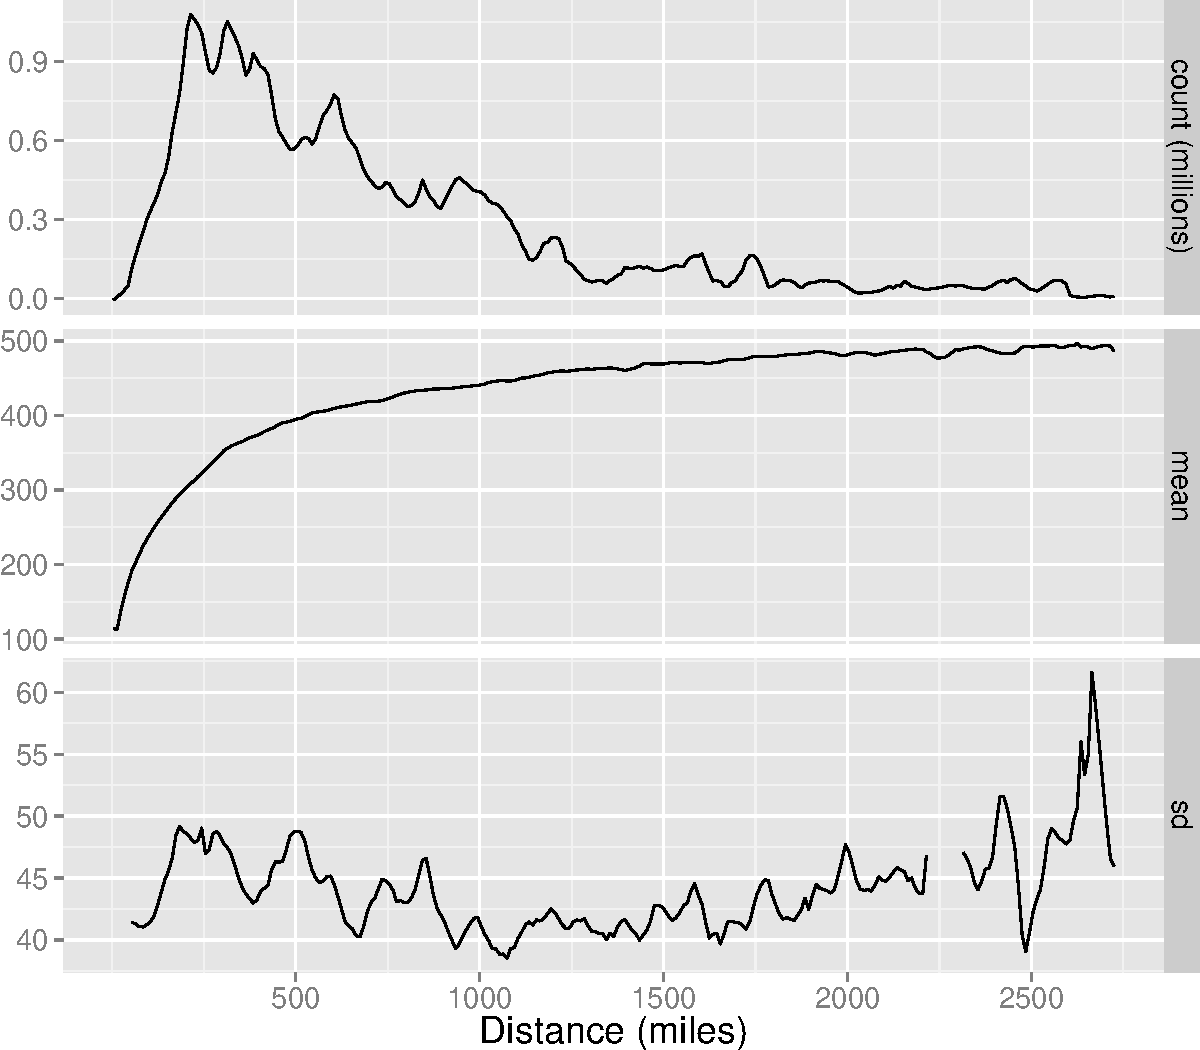
\includegraphics[width=\linewidth]{smooth}
 \caption{The same underlying data from Figure~\ref{fig:condense}, but smoothed with a bandwidth of 50. This removes much of the uninteresting variation while preserving the main trends.}
 \label{fig:smooth}
\end{figure}

There are many approaches to smoothing, but we use a family of kernel based methods, because they:

\begin{itemize}
  \item are simple and efficient to compute,
  
  \item have a single parameter, the {\bf bandwidth} that controls the amount of smoothing,

  \item work equally well when applied to binned data \cite{wand:1994},
  
  \item are approximately equivalent to other more complicated types of smoothing \citep{silverman:1984}, 
  
  \item form the heart of many existing statistical visualisations such as the kernel density plot \citep{scott:1992}, average shifted histogram \citep{scott:1985} and loess \citep{cleveland:1979}.

\end{itemize}

\subsection{How it works}

Figure~\ref{fig:smooth-types} illustrates the progression of smoothing methods from fast and crude to sophisticated and slow. The simplest smoothing method (top) is the binned mean, where we divide the data in bins and compute the mean of each bin. This is simple, but is locally constant and not very smooth. The next step up in complexity is the running (or nearest neighbour) mean where we average the five nearest points at each location.  This is a considerable improvement, but is still rather jagged.

\begin{figure}[htb]
 \centering
 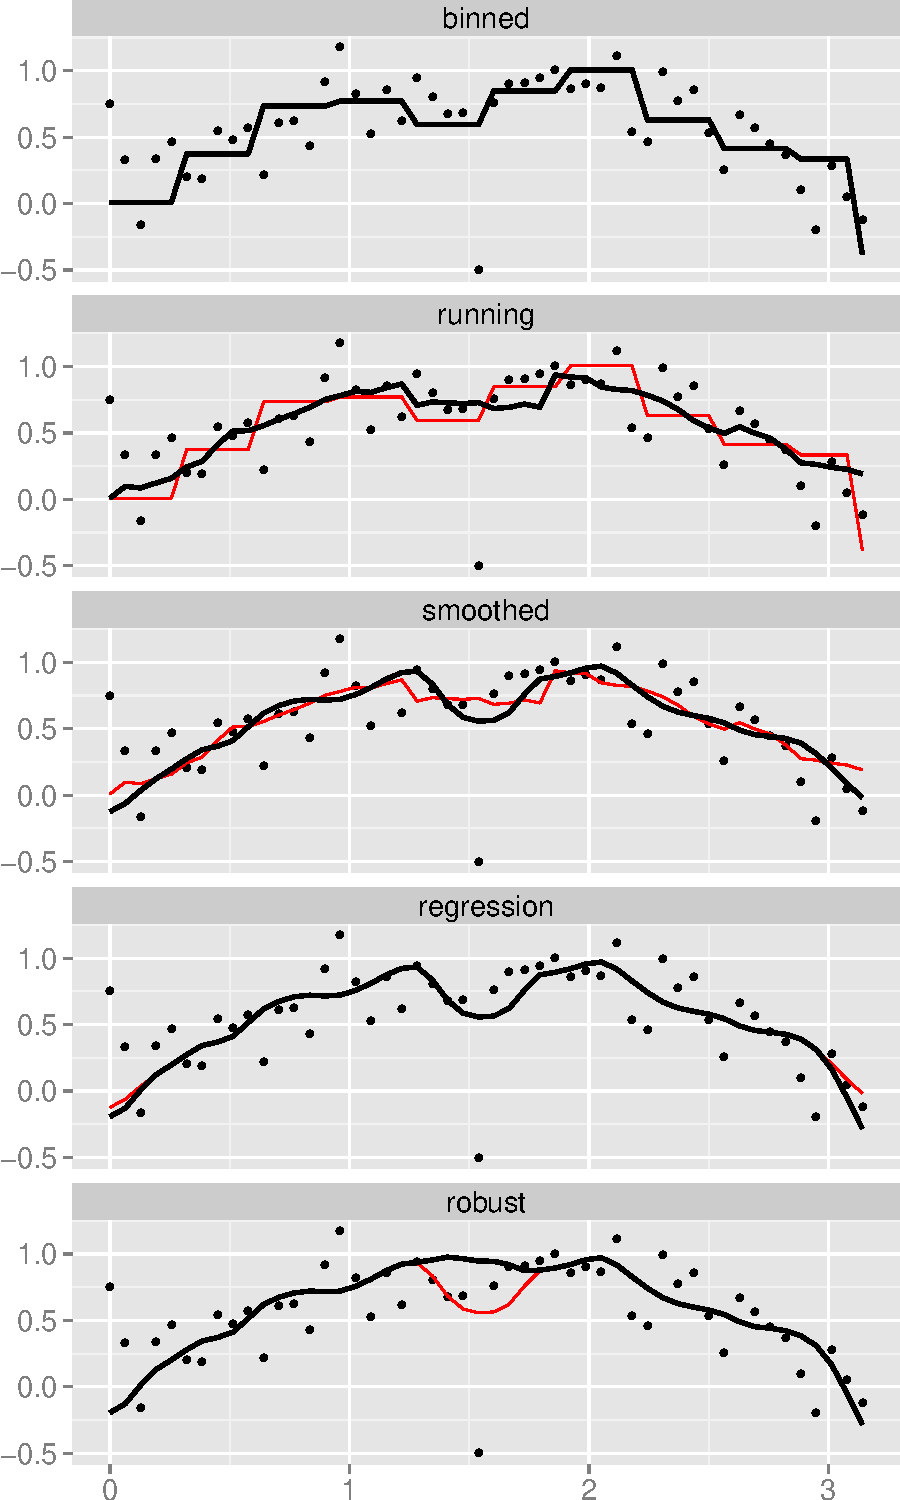
\includegraphics[width=0.75\linewidth]{smooth-types}
 \caption{Five types of smoothing on a artificial dataset generated with $\sin(x)$ on $[0, \pi]$, with random normal noise with $\sigma = 0.2$, and an outlier at $\pi / 2$. Smoothes are arranged from simplest (top, binned) to most accurate (bottom, robust local regression). To aid comparison each smooth is shown twice, prominently with a thick black line, and then repeated on the next plot in red to make comparison easier. The subtlest difference is the between the kernel mean and kernel regression: look closely at the boundaries.}
 \label{fig:smooth-types}
\end{figure}

The remaining three types use a simple idea: we want to not only use the neighbouring points, but we want to weight them according to their distance from the target point. In statistics, the weighting function is traditionally called a {\bf kernel}. Many kernels are available, but there is little evidence to suggest that the precise form of the kernel is important \citep{cleveland:1996}. Gaussian kernels are common, but I recommend the triweight, $K(x) = (1 - |x|^3)^2 I_{|x| < 1}$, because it is bounded and simple (evaluation of this function is $\sim 10 \times$ faster than evaluation of a Gaussian).  

At each binned location we have $x_i$, the center of the bin, $y_i$ the summary of that bin and $w_i$ the number of observations in that bin. To predict a smooth estimate at position $j$, we first compute the kernel weights for each location $k_i = K(\frac{x_j - x_i}{h})$. The parameter $h$ is called the bandwidth, and controls the degree of smoothing: the larger $h$ is, the more neighbours are used to compute the smooth and the smoother the final curve. Because of the form of the triweight kernel, any observation more than $h$ away from $x_j$ will not contribute to the smoothed value, thus enabling efficient computation.

The three kernel techniques, kernel means (aka Nadaraya-Watston smoothing), kernel regression (aka local regression) and robust kernel regression (aka loess), make a tradeoff between performance and quality. They improve upon the simple runing mean and provide a smooth tradeoff of computational vs.\ statistical performance. While closely related, these methods developed in different parts of statistics at different times, and the terminology is often inconsistent. I have attempted to provide a unifying description here; \citep{cleveland:1996} provides a good historical overview of kernel smoothing methods.

The kernel (weighted) mean is fastest to compute but suffers from bias on the boundaries, because the neighbours only lie on one side. The kernel (weighted) regression overcomes this problems by effectively using a first-degree Taylor approximation. In Figure~\ref{fig:smooth-types}, you can see that the kernel mean and kernel regression are coincident everywhere except near the boundaries. Higher-order approximations can be used (by fitting higher order polynomials in the model), but there seems to be little additional benefit in practice \citep{cleveland:1996}.

Finally, the robust kernel regression iteratively down-weights the effect of points far away from the curve, and reduces the impact of unusual points at the cost of increased computation time. In Figure~\ref{fig:smooth-types} observe that the kernel robust regression is the only smoother unaffected by the unusually low point at $\pi / 2$.

\subsection{High-dimensions and performance characteristics}

The three kernel techniques are readily extended to higher dimensions, using corresponding higher dimensional means and regressions. Optimisations are also available. Kernel weighted means are particularly easy to efficiently extend to higher dimensions  because they are a convolution, and due to the associative nature of convolution it's possible to perform an nD smooth through a sequence of 1d kernel smooths. This is an important optimisation because it converts an $O(n^d)$ process to $O(nd)$.  You can treat local regression in a similar way, although it is only approximate if the grid of values is not uncorrelated. Approximate robust local regression does not work.

While the fast fourier transformation is a common technique to speed up discrete convolution, it is not effective here.  Using the FFT makes code considerably more complicated (extra padding is needed to avoid the periodic nature of the FFT), and less flexible. Direct convolution with nested loops also makes it easier to predict smoothed values at specified locations, which it useful for cross-validation.

\subsection{Kernel density estimates vs.\ kernel smoothed counts}

Note that when applied to count summaries, these methods are subtly different from a kernel density estimate. A kernel mean is similar to a kernel density estimate: but a kernel mean divides by (normalises by) by the total weight at each point. This change is most noticeable with small bandwidths: the kernel density estimates will be very large (because they must integrate to 1), and outside the range of the data the estimates will be 0, where outside the range of the data the smoothed counts will be undefined (0/0).

\subsection{``Automatic'' bandwidth selection}

Kernel smoothing introduces a tuning parameter: the bandwidth. There is much research on how to pick the ``best'' bandwidth, but it depends critically on what measurement of quality and the specific type of smoothing. Typically, integrated mean squared error is used, which may not correspond with what we actually want for visualisation \citep{denby:2009}. We take a pragmatic attitude and use leave-one-out cross-validation (loocv) \citep{efron:1983} to provide a starting point for the user. This is supported by \citep{loader:1999}, which finds that plug-in methods often do not live up to their asymptotic claims.

The intution behind loocv is simple: we compare the actual statistic at a location with its smoothed estimate computed without that observation. We then summarise all errors using the root mean squared error (rmse): $\sqrt{ \sum (y_i - \hat{y}_i)^2 / n}$. We can explore this summary across a range of possible grid values, or use standard numerical optimisation (L-BFGS-B \citep{byrd:1995}). While this is a good starting point, and is optimal in the sense of predicting new values, in our experience, this procedure tends to pick a bandwidth that is too small, preserving features in the data that while may be important, distract from the overall picture.

With the bounded tricube kernel, this is straightforward to implement efficiently, in $O(m b)$ where $b$ is the number of bins covered by the kernel ($b \ll m$). \citep{fan:1994} suggests incremental algorithms that may reduce computation time still further.

\subsection{Varying bandwidths}

Intuitively, it seems like we should be able to do better with an adaptive binwidth: using small bins where there is more data, or where the curve is especially wiggly. There are many approaches documented in the literature  \citep{terrell:1992, brockmann:1993,schucany:1995,herrmann:1997}. We follow the simple, but performant, approach outlined in \citep{fan:1995}: to find a per-location $h$, we divide the data into $m / (10 * \log(m))$ pieces, estimate the optimal bandwidth for each piece separately, then smooth the estimates.

Figure~\ref{fig:varying-h} illustrates the process for a challenging function proposed by \citep{fan:1995}. 

\begin{figure*}[htb]
 \centering
 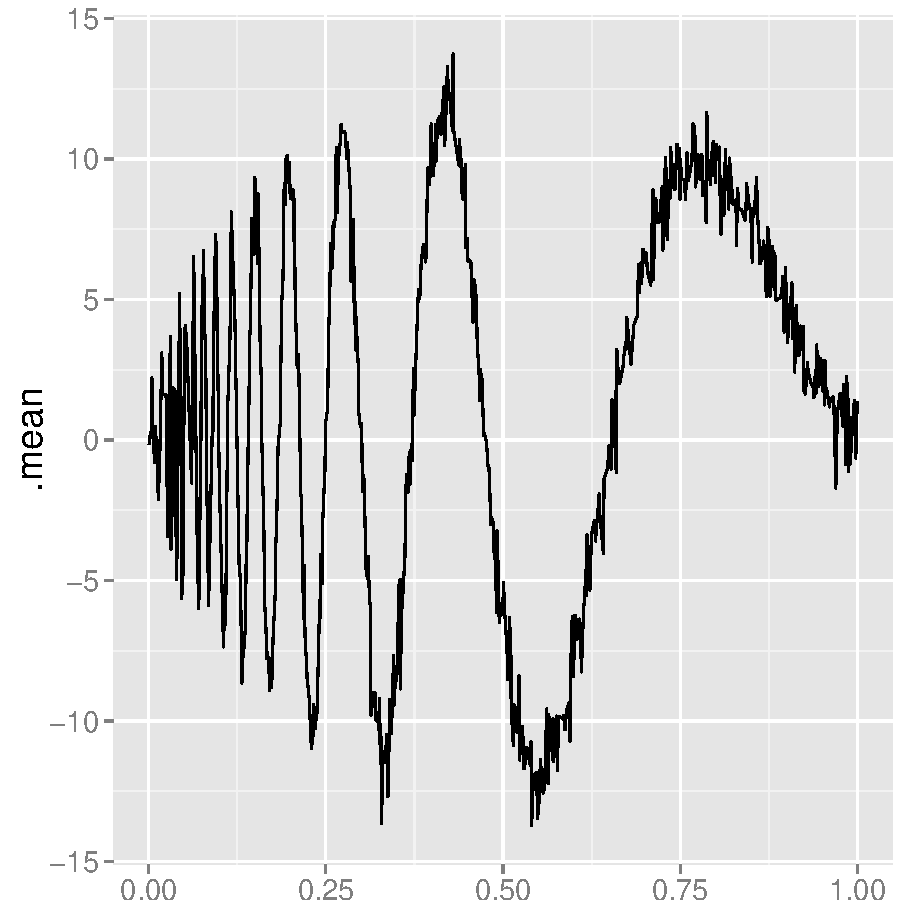
\includegraphics[width=0.25\linewidth]{variable-h-raw}%
 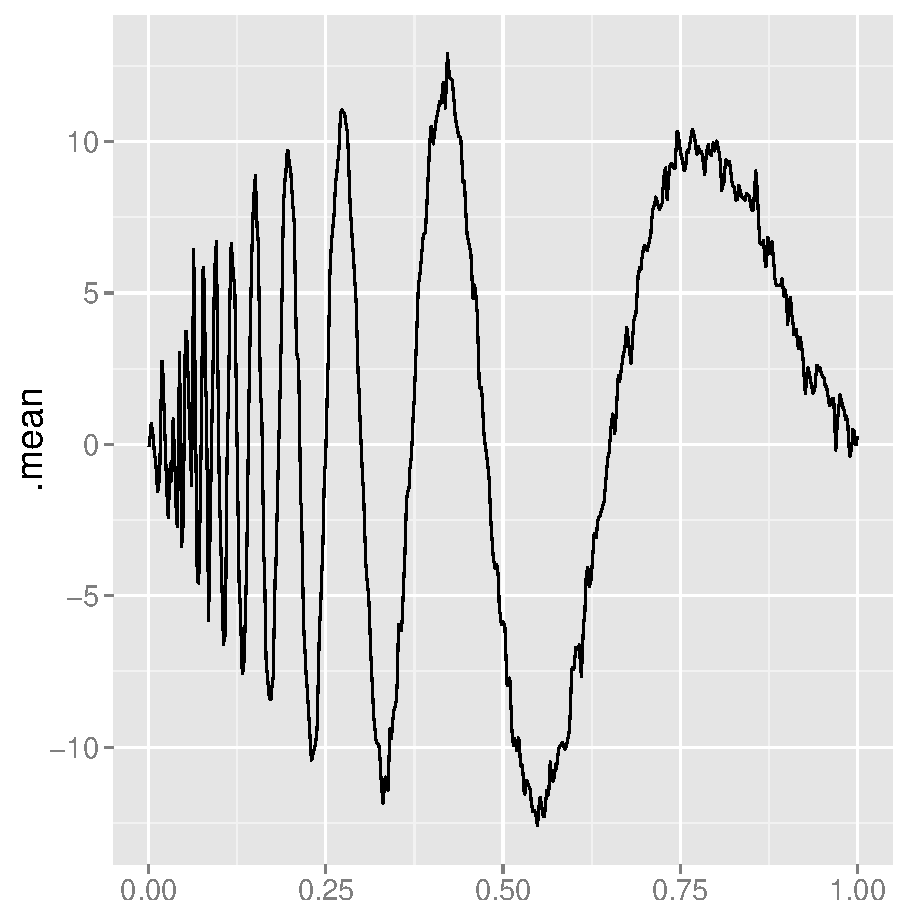
\includegraphics[width=0.25\linewidth]{variable-h-smoothed-fixed}%
 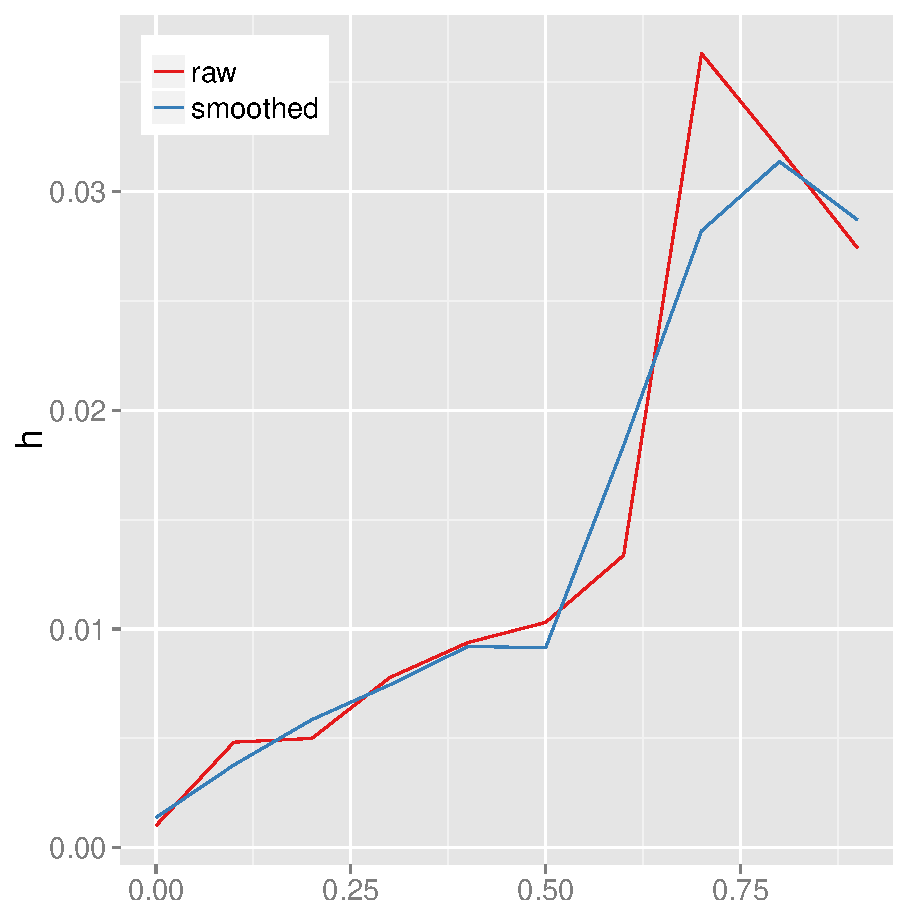
\includegraphics[width=0.25\linewidth]{variable-h-h-est}%
 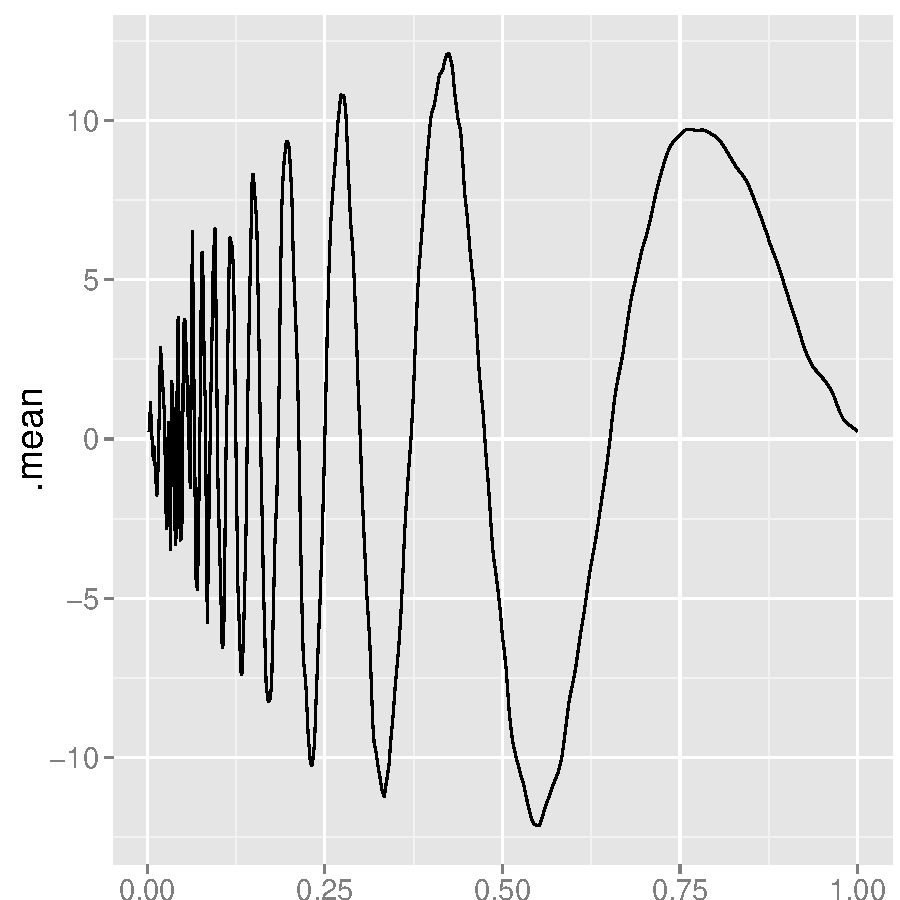
\includegraphics[width=0.25\linewidth]{variable-h-smoothed-var}%
 \caption{(Far left) A challenging function to smooth with fixed bandwidth \citep{fan:1995}. (Left) Data smoothed using single best bandwidth. (Right) Optimal bandwidth estimated on 10 separate pieces. (Far right) Data smoothed using individual bandwidth at each location.}
 \label{fig:varying-h}
\end{figure*}

\section{Visualise}
\label{sec:visualise}

Relatively straightforward to visualise the resulting data, but we discuss a number of important issues to consider both statistically and visually.  Figure~\ref{fig:vis-types} illustrates the basic types of graphics for 1d and 2d summaries. Visualising counts vs. visualising other summary statistics.  Important to distinguish because all other summaries must be read taking into account how much underlying data there is: you don't want to draw conclusions about areas that have relatively few data points.

Note that for a 1d summary of counts we use a frequency polygon \citep{scott:1985a}, where the centers of each bar are connected with a line. This unifies the display of counts and other summaries; makes it easier to overlay multiple distributions (if summarised by another categorical variable); and asymptotic arguments suggest that it has slightly lower error than a histogram.

\begin{table}
  \scriptsize
  \centering
  \begin{tabular}{lll}
  \toprule
  Dimension & Count & Other summary\\
  \midrule
  1d & Frequency polygon & Line plot \\
  2d & Heatmap, Contour plot, Hypsograph & Heatmap + alpha\\
  \bottomrule
  \end{tabular}
  \caption{Basic visualisation components}
  \label{fig:vis-types}
\end{table}

On top of these basic plots, we add three suggested design principles for visualisation of large datasets:

\begin{itemize}
  \item Preserve missing values
  \item Prepare for outliers
  \item Display uncertainty
\end{itemize}

The product plots \citep{me:prodplots} framework provides a way of generalising these plots to higher dimensions, and for integrating with other categorical variables. For count data, we can draw on insights from . Once continuous data has been binned, it can be treated the same way as discrete data and it falls naturally into the framework of product plots. A small additioanl constraint is that only the final level can been a continuous display; which implies that even if higher levels are continuous they are coarsely binned .  It is also interesting to think about the limit of plots as the number of bins goes to infinity.  The product plots framework shows how these ideas can be adapted to display arbitrary dimensions.

\subsection{Missing values}

Another design principle (inspired by that of R) is that missing values should never be omitted without user intervention: they should always be preserved along the entire route from raw data to final visualisation. It is possible to remove them, but it must be a deliberate decisions: you never want to inadvertently distort your visualisations by silently leaving off data.

This principle also needs to be carried through all other components of the framework - missing values must be correctly binned, summarised and smoothed.

\subsection{Missing values}

As the size of data grows, the probability of finding very unusual values also grows. In practice, we have found the visualisation of most large datasets look like Figure~\ref{fig:teaser} - most of the data is concentrated in a relatively small error of the plot. We have two tools to deal with this: peeling, when the outliers are spatial; and the modulus transformation, when the outliers are in colour, size or another aesthetic.

\subsubsection{Peeling}

A simple approach to deal with spatial outliers is to remove the smallest outer values. We call this approach peeling, and have implemented it by progressively removing the smallest counts on the convex hull of the dataset.

Typically, you don't want to ignore these unusual values, but instead you partition your analysis to look at the most common and at the unusual. Some small amount of peeling (often $< 1\%$) seems to improve most 2d plots, drawing the focus to the bulk of the data.  For plots of non-count summaries, this also has the additional benefit of reducing outliers in the summary dimension. 

\subsubsection{Modulus transformation}
\label{sub:transform}

The modulus transformation \citep{john:1980} is a generalisation of the box-cox transformation \citep{box:1964} to deal with positive and negative data. It provides a flexible tool to shrink or expand the tails of a distribution.

\begin{equation}
\begin{cases} 
  \text{sgn}(x) \cdot \log(|x| + 1) & \text{if $\lambda = 0$,} \\
  \text{sgn}(x) \cdot \frac{(|x| + 1)^\lambda - 1}{\lambda} &\text{if $\lambda \ne 0$.}
\end{cases}
\end{equation}

This transformation is particularly useful in conjunction with interactivity, as it allows the use to dynamically focus on important parts of the distribution.

\subsection{Error}

Vital that these displays

\section{The {\tt bigvis} package}
\label{sec:bigvis}

The bigvis package demonstrates the ideas discussed in this paper in an open-source R package available from \url{http://github.com/hadley/bigvis}. It has two main parts: a high-performance implementation of the key algorithms written in C++ and a flexible, user-friendly wrapper that supports exploratory data analysis written in R. The key to bridging the two pieces is the Rcpp package \citep{eddelbuettel:2011} which provides an easy way to access R's internal datastructures with a clean C++ API. 

The C++ component makes use of templated functions to avoid the cost of virtual method lookup (this is small, but adds up with potentially 100's of millions of invocations). This adds an additional challenge when connecting R and C++ because templated functions are specialised at compile time, but the R code needs to call them dynamically at run-time. To work around this problem, a small code generater generates all specialised versions of templated functions. This is somewhat inelegant, but unavoidable when coupling programming languages with such different semantics.

The bigvis {\sc api} is designed to make visualisation large datasets familiar to R users. It implements methods of the {\tt autoplot} generic providing default visualisations designed using the principles above, and also cleanly interfaces with other plotting tools in R, like ggplot2 \citep{me:ggplot2,wickham:2007d}, which makes it easy to build custom graphics based on the condensed and smoothed data.

The reference implementation provides some of the constraints that guide this paper. It is designed to be used by experienced analysts who will be using  sophisticated statistical and machine learning models in conjunction with visualisation.  It allows the analyst to create plots of $10^8$ observations in under 5s. $10^8$ doubles occupy a little less than 800 Mb, so about 20 vectors can be stored in 16 Gb of ram, with about 1 Gb left over. Support tiered model of data access: analyst may have access to billions or trillion of observation in a multi-machine data warehouse, but for most problems some interactive exploration is needed on a small subset or aggregate. 5s is an interactive timeframe for a REPL.  This is arbitrary but is currently about how long it takes to draw a scatterplot of 200,000. It's well above the threshold for direct manipulative interaction, but my personal experience seems to be on the order of what I expect when doing interactive data analysis in R.  Too much longer and I start checking my email and my productivity goes down hill.

\subsection{Benchmarks}
\label{sub:benchmarks}

A back-of-the-envelope calculation gives us a performance target: assuming we want to condense 100 million observations into 10,000 bins in under 5s, we need to be able to compute each summary of 10,000 observations in 0.5 ms, which implies we have no more than 50 ns to process each observation. This is achievable with a high-performance language like C++. In the reference implementation, summarising $10^8$ observations in $10^4$ bins takes $\sim 2.8$s for the mean, $\sim 3$s for the variance, and $\sim 5.8$s the median. \footnote{Timings performed on a 2.6 GHz Intel Core i7, 15\" MacBook retina} \footnote{These are likely to be upper bounds as I have only programmed in C++ for 6 months, and did not use any performance tricks}.  More details are provided in Section~\ref{sub:benchmarks}.


C++ is extremely efficient and the data structures and algorithms provided by the STL make programming considerably faster.  The C++ code is by no means expert and uses only a smattering of advanced C++ functions; I have been programming in C++ for less than six months. There are likely to be considerable opportunities for further optimisation.

These benchmarks ignore the time needed to load the data into R, which is on the order of 3-5 seconds once it has been serialised in R's binary dataformat.  Unfortunately due to inefficiencies in the implementation of R's data frame strucutre, data frames can not be used to work with very large vectors without substantial performance penalities. Future work will hopefully address some of the deficiencies in R's data model and make it easier to work with large datasets.


% \begin{figure}[htb]
%  \centering
%  \includegraphics[width=1.5in]{sample}
%  \caption{Sample illustration.}
% \end{figure}

\section{Future work}
\label{sec:conclusion}

While the reference implementation is in-memory and single-core, parallelisation and out-of-memory datastores are obvious areas for future work. We expect that fine pre-binning with simple summaries may be done in existing datastore; the grouping algorithm is trivial to implement in SQL, and most databases already provide simple summary statistics like the mean. Other systems, e.g.\ madlibs \citep{hellerstein:2012}, may provide richer summaries making grouping and summarisating in the database even more appealing. However, databases are is likely to be high-throughput and higher-latency than local computing. This suggests a workflow where we supplement fine prebinning in the database with coarser binning locally, especially when supporting interactive graphics.

Something about column stores: \citep{kersten:2011}

Categorical data: prebinned, and can't be be smoothed.

Visualisation is only one piece of the data analysis puzzle: we also need tools for transforming and modelling big data. 

%% if specified like this the section will be committed in review mode
\acknowledgments{
The authors wish to thank Yue Hue who coded up many of the initial prototypes. And to JJ Allaire, Dirk Eddelbuettel, Romain Francois and Carlos Scheidegger for their help with C++. Early versions of this work were generously sponsored by Revolution Analytics.}

\bibliographystyle{abbrv}
% bibtool -x bigvis > references.bib

\bibliography{references}
\end{document}
